\documentclass[11pt,oneside,draft]{amsart}
\usepackage[T1]{fontenc}
\usepackage[english]{babel}
\usepackage{fouriernc} % Fourier fonts instead of Computer Modern

\usepackage{geometry} % page geometry
\usepackage{xcolor} % colors
\usepackage{tikz} % drawing
\usepackage{hyperref} % hyperlinks

\usepackage{amsmath,amsthm,amssymb}
\usepackage[all,cmtip]{xy}



%%
%% cross references
%%
\usepackage[capitalise]{cleveref}  % load after hyperref
\newcommand{\clevertheorem}[3]{%
  \newtheorem{#1}[thm]{#2}
  \crefname{#1}{#2}{#3}
}


%% Makes equations appear as secno.eqno
\numberwithin{equation}{section} %% Comment out for sequentially-numbered
\numberwithin{figure}{section} %% Comment out for sequentially-numbered


%%
%% theorem-like environments
%%
\theoremstyle{plain} % bold environment name, italic text
\newtheorem{thm}{Theorem}[section]
\crefname{thm}{Theorem}{Theorems}
\newtheorem*{thm*}{Theorem}
\clevertheorem{prop}{Proposition}{Propositions}
\newtheorem*{prop*}{Proposition}
\clevertheorem{lem}{Lemma}{Lemmas}
\clevertheorem{cor}{Corollary}{Corollaries}
\clevertheorem{conj}{Conjecture}{Conjectures}

\theoremstyle{definition} % bold environment name, plain text
\clevertheorem{defn}{Definition}{Definitions}
\clevertheorem{notn}{Notation}{Notations}

\theoremstyle{remark} % italic environment name, plain text
\clevertheorem{rmk}{Remark}{Remarks}

\newtheorem*{note}{Note}

%% This makes equations follow the theorem counter
\makeatletter\let\c@equation\c@thm\makeatother
%% This makes figures follow the theorem counter
\makeatletter\let\c@figure\c@thm\makeatother


% Additional cleveref definitions
\crefname{figure}{Figure}{Figures}
\crefname{equation}{Display}{Displays} % give 'equation' a more general name 
\crefname{eq}{Display}{Displays}
\crefname{eqn}{Display}{Displays}



%%
%% Document-specific stuff
%%


%% document-specific options for hyperref
\hypersetup{
 pdfkeywords={latex starter,template},
 pdfauthor={Niles Johnson},
}



%% MSC
%% http://www.ams.org/mathscinet/msc/msc2010.html
\subjclass[2010]{55P42}

% 55P42 Stable homotopy theory, spectra
% 55N15 K-theory
% 18D10 Monoidal categories
% 18D05 Double categories, 2-categories, bicategories
% 19D23 Symmetric monoidal categories (in K-theory)
% 

\title{A Latex package demo}

\author{Your Name}
\address{Your Address}
\email{you@example.com}
\urladdr{\url{http://nilesjohnson.net}}

\date{\today}

\begin{document}

\begin{abstract}
  This is a latex starter for It is based on the template developed for the REU
  program at the University of Chicago.
\end{abstract}

\maketitle

\tableofcontents

\section{What does the table of contents command do?}

The table of contents command will automatically make a contents; if
your document is short, you probably don't need a table of contents.
You must run tex at least twice for this to work.

\section{How do the environment commands work?}\label{env-commands}

``Environments'' are commands that are given using the \verb|\begin{}|
  and \verb|\end{}| syntax. In the preamble, you can see we've defined
  a bunch of theorem-type environments, including, for example ``\texttt{defn}'' To get a definition, 
you type:

\begin{defn}  This is how to define a definition.
\end{defn}

And for a theorem and its proof you would type:

\begin{thm}\label{atheorem}
This is the statement of a theorem.
\end{thm}
\begin{proof}
And this shows that the statement is correct.
\end{proof}

Note that the numbering is taken care of automatically, and that we've predefined a bunch of these sorts of environments to take care lemmas, corollaries and such in the header. 

\subsection{Displaying equations}
Another useful kind of enviroment is the equation environment.  Equations
get numbered in sequence with statements, as for example

\begin{equation}\label{eq1}  e = mc^2
\end{equation}

Note if you do not want a numbered equation, you can use the
environment ``\texttt{equation*}''
 like so:

\begin{equation*}
e=mc^2
\end{equation*}

For multiline equations, use ``\texttt{align}'' or
``\texttt{align*}'':

\begin{align}
  (x + y)^2 & = (x+y) (x+y) \label{eq2}\\
  & = x(x+y) + y(x+y) \nonumber\\
  & = x^2 + xy + yx + y^2 \label{eq3}
\end{align}

There are plenty of other equation-type enviroments that allow you to
align several equations and such. The AMS's guide \cite{amsshort} is a
good place to start with these.


\subsection{Inline math mode}
You can also typeset math directly in a paragraph by placing it within
\$dollar signs\$ or \verb|\(|backslash round brackets\verb|\)|.  This is called ``inline math mode.''  For example: Let $e$
be energy, $m$ be momentum and $c$ be the speed of light.  Then
Einstein's famous equation says that \(e=mc^2\).  You should use inline
math mode whenever you use a variable name or math symbol in text.
This distinguishes variables $a$ or $i$ from words such as a or i.
For longer equations, you should use ``display math mode''.

\subsection{Display math mode}
Displayed math is typset on a separate line, and centered, such as
\[
e = mc^2.
\]
To display math, enclose it in \verb|\[|backslash square
brackets\verb|\]|.  Remember that you should include appropriate punctuation in
displayed math.

\subsection{Symbols}

Both \cite{notsoshort} and \cite{amsshort} have good lists of symbols
you can use in math mode.  These include greek letters ($\alpha,
\beta, \Gamma, \Delta$), operators ($\otimes, +, \sum$) and much more
($\leq, \diamond$).  Note that some symbols are slightly different
depending on whether they are used inline or displayed.


\subsection{Further comments on text}

If you want to \emph{emphasize} something in your text, use
\verb|\emph{}|.  For \textbf{boldface}, \textit{italics},
\texttt{monospace}, and \textsc{smallcaps}, use \verb|\textbf{}|
\verb|\textit{}|, \verb|\texttt{}|, and \verb|\textsc{}|.  These
should be used \emph{very sparingly}.  

Also note the formatting of ``quotation marks'' -- this requires using
\verb|``| (two backticks) to open the quotation, and a usual quotation
mark (or two apostrophes) to close.  If you just use the quotation
mark key on your keyboard, you'll get something that ''looks silly''.

Cross-references are produced with \texttt{label/ref} pairs.  Put
\verb|\label{somename}| next to what you want to reference, and then
use \verb|\ref{somename}| to reference that item.  For example, the
section on environment commands is \ref{env-commands}, and it contains
a theorem numbered \ref{atheorem}.  Latex must be run twice to
correctly detect and print cross-references.

The \texttt{cref} package provides the command \verb|\cref|, which
automatically includes the name of the environment.  So you can
refer to \cref{atheorem} or \cref{env-commands}.  It also
properly handles multiple references, such as \cref{eq1,eq3}.

\section{Xypic and diagrams}

If you want to draw diagrams, you could use xypic.  It's actually
much easier than it looks, and we've already included it in the header
above.  Here is an example. 
\[\xymatrix{
FX \ar[r]^-{Ff} \ar[d]_{\eta_X} & FY \ar[d]^{\eta_Y} \\
GX \ar[r]_-{Gf} & GY\\} \]

\section{TikZ for more complex drawings}

TikZ is somewhat more full-featured than xypic.  It has an extensive
manual, a large online community, and a steep learning curve.  Here's one
example diagram:

\begin{center}
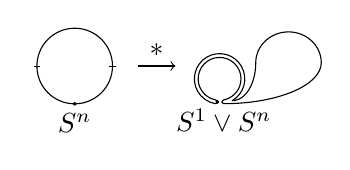
\begin{tikzpicture}[scale=.8]
  \draw (-2.5,-.05) node (t) {} 
  arc(-90:0:.6cm) node (h1) {}
  arc(0:180:.6cm) node (h2) {}
  arc(180:270:.6cm);
  \draw[fill=black] (t) circle (.02);
  \draw[very thin] (h1) ++(-.05,0) -- ++(.1,0);
  \draw[very thin] (h2) ++(-.05,0) -- ++(.1,0);

  \draw (t) ++(0,-.3cm) node {$S^n$};

  \draw[->] (t) ++(1cm,.6cm) -- node[above]{$*$}++(.6cm,0);
  \draw[cap=round,join=round] (0,0) 
  arc(-60:260:.4cm) 
  arc(-100:0:.03cm)
  node(x){}
  arc(0:80:.03cm)
  arc(260:-80:.34cm)
  arc(100:270:.03cm)
  arc(-90:0:1.55cm and .65cm)
  arc(0:180:.52cm and .49cm)
  arc(0:-85:.367cm and .602cm)
  --cycle;

  \draw[fill=black] (x) circle(.02);
  \draw (x) ++(.1cm,-.3cm) node{$S^1 \vee S^n$};
\end{tikzpicture}
\end{center}


\subsection*{Acknowledgments}  

This document began as a template for REU students at the University
of Chicago.  Further improvements were made by Anna Marie Bohmann.
Niles Johnson made some other additions and modified it for a wider
audience.

\begin{thebibliography}{9}

\bibitem{amsshort}
Michael Downes.
Short Math Guide for \LaTeX.
ftp://ftp.ams.org/pub/tex/doc/amsmath/short-math-guide.pdf

\bibitem{May}
J. P. May.
A Concise Course in Algebraic Topology.
University of Chicago Press. 1999. 

\bibitem{notsoshort}
Tobias Oekiter, Hubert Partl, Irene Hyna and Elisabeth Schlegl.
The Not So Short Introduction to \LaTeXe.
http://tobi.oetiker.ch/lshort/lshort.pdf.

\end{thebibliography}

\end{document}

